% This LaTeX was auto-generated from MATLAB code.
% To make changes, update the MATLAB code and export to LaTeX again.

\documentclass{article}

\usepackage[utf8]{inputenc}
\usepackage[T1]{fontenc}
\usepackage{lmodern}
\usepackage{graphicx}
\usepackage{color}
\usepackage{hyperref}
\usepackage{amsmath}
\usepackage{amsfonts}
\usepackage{epstopdf}
\usepackage[table]{xcolor}
\usepackage{matlab}
\usepackage{geometry}

\geometry{
	paper=a4paper, 
	top=2.5cm,
	bottom=2.5cm, 
	left=2.5cm, 
	right=3cm
}

% \sloppy
\epstopdfsetup{outdir=./}
\graphicspath{ {./ME331_HW13_ex_images/} }

\begin{document}
\begin{matlabcode}
% 11811126 Zhuang Yulun
close all;clear;clc;
\end{matlabcode}


\matlabheading{Phase 1}

\begin{matlabcode}
%% Phase 1
syms m L I a q dq [1 3]
syms r g
n = 3;
m = m.';
L = L.';
I = I.';
a = a.';
q = q.';
dq = dq.';

p = cell(n,1);
p{1} = [-(a(1)-r)*sin(q(1)),-(a(1)-r)*cos(q(1))];
p{2} = [-(L(1)-r)*sin(q(1))-a(2)*sin(q(2)),...
        -(L(1)-r)*cos(q(1))-a(2)*cos(q(2))];
p{3} = [-(L(1)-r)*sin(q(1))-L(2)*sin(q(2))-a(3)*sin(q(3)),...
        -(L(1)-r)*cos(q(1))-L(2)*cos(q(2))-a(3)*cos(q(3))];

v = cell(n,1);
K = 0;
P = 0;
for i = 1:n
    v{i} = jacobian(p{i},q)*dq;
    v{i}(1) = v{i}(1)+ r*dq1;
    K = K+1/2*m(i)*v{i}.'*v{i}+1/2*dq(i).'*I(i)*dq(i);
    P = P+m(i)*g*p{i}(2); 
end

K = simplify(expand(K));
P = simplify(expand(P));

D = jacobian(K,dq).';
D = jacobian(D,dq);

G = jacobian(P,q).';

syms C real
for k=1:n
	for j=1:n
        C(k,j)=0;
        for i=1:n
            C(k,j)=C(k,j)+(1/2)*(jacobian(D(k,j),q(i))...
            +jacobian(D(k,i),q(j))-jacobian(D(i,j),q(k)))*dq(i);
        end
	end
end
D1 = simplify(expand(D));
C1 = simplify(expand(C));
G1 = simplify(expand(G));
disp(D1)
\end{matlabcode}
\newpage
\begin{matlabsymbolicoutput}
\hskip1em $\displaystyle \begin{array}{l}
\left(\begin{array}{ccc}
I_1 +{L_1 }^2 \,m_2 +{L_1 }^2 \,m_3 +{a_1 }^2 \,m_1 +2\,m_1 \,r^2 +2\,m_2 \,r^2 +2\,m_3 \,r^2 +2\,m_1 \,r^2 \,\\
\cos \left(q_1 \right)+2\,m_2 \,r^2 \,\cos \left(q_1 \right)+2\,m_3 \,r^2 \,\\
\cos \left(q_1 \right)-2\,L_1 \,m_2 \,r-2\,L_1 \,m_3 \,r-2\,a_1 \,m_1 \,r-2\,L_1 \,m_2 \,r\,\\
\cos \left(q_1 \right)-2\,L_1 \,m_3 \,r\,\cos \left(q_1 \right)-2\,a_1 \,m_1 \,r\,\cos \left(q_1 \right) & \sigma_1  & \sigma_2 \\
\sigma_1  & m_3 \,{L_2 }^2 +m_2 \,{a_2 }^2 +I_2  & \sigma_3 \\
\sigma_2  & \sigma_3  & m_3 \,{a_3 }^2 +I_3 
\end{array}\right)\\
\mathrm{}\\
\textrm{where}\\
\mathrm{}\\
\;\;\sigma_1 =-{\left(L_2 \,m_3 +a_2 \,m_2 \right)}\,{\left(r\,\cos \left(q_2 \right)-L_1 \,\cos \left(q_1 -q_2 \right)+r\,\cos \left(q_1 -q_2 \right)\right)}\\
\mathrm{}\\
\;\;\sigma_2 =-a_3 \,m_3 \,{\left(r\,\cos \left(q_3 \right)-L_1 \,\cos \left(q_1 -q_3 \right)+r\,\cos \left(q_1 -q_3 \right)\right)}\\
\mathrm{}\\
\;\;\sigma_3 =L_2 \,a_3 \,m_3 \,\cos \left(q_2 -q_3 \right)
\end{array}$
\end{matlabsymbolicoutput}
\begin{matlabcode}
disp(C1)
\end{matlabcode}
\begin{matlabsymbolicoutput}
\hskip1em $\displaystyle \begin{array}{l}
\left(\begin{array}{ccc}
{\textrm{dq}}_1 \,r\,\sin \left(q_1 \right)\,\\
{\left(L_1 \,m_2 +L_1 \,m_3 +a_1 \,m_1 -m_1 \,r-m_2 \,r-m_3 \,r\right)} & {\textrm{dq}}_2 \,\sigma_1 \,\\
{\left(r\,\sin \left(q_2 \right)+L_1 \,\sin \left(q_1 -q_2 \right)-r\,\sin \left(q_1 -q_2 \right)\right)} & a_3 \,\\
{\textrm{dq}}_3 \,m_3\\
 \,{\left(r\,\sin \left(q_3 \right)+L_1 \,\sin \left(q_1 -q_3 \right)-r\,\sin \left(q_1 -q_3 \right)\right)}\\
-{\textrm{dq}}_1 \,\sin \left(q_1 -q_2 \right)\,{\left(L_1 -r\right)}\,\sigma_1  & 0 & L_2 \,a_3 \,{\textrm{dq}}_3 \,m_3 \,\sin \left(q_2 -q_3 \right)\\
-a_3 \,{\textrm{dq}}_1 \,m_3 \,\sin \left(q_1 -q_3 \right)\,{\left(L_1 -r\right)} & -L_2 \,a_3 \,{\textrm{dq}}_2 \,m_3 \,\sin \left(q_2 -q_3 \right) & 0
\end{array}\right)\\
\mathrm{}\\
\textrm{where}\\
\mathrm{}\\
\;\;\sigma_1 =L_2 \,m_3 +a_2 \,m_2 
\end{array}$
\end{matlabsymbolicoutput}
\begin{matlabcode}
disp(G1)
\end{matlabcode}
\begin{matlabsymbolicoutput}
\hskip1em $\displaystyle \left(\begin{array}{c}
g\,\sin \left(q_1 \right)\,{\left(L_1 \,m_2 +L_1 \,m_3 +a_1 \,m_1 -m_1 \,r-m_2 \,r-m_3 \,r\right)}\\
g\,\sin \left(q_2 \right)\,{\left(L_2 \,m_3 +a_2 \,m_2 \right)}\\
a_3 \,g\,m_3 \,\sin \left(q_3 \right)
\end{array}\right)$
\end{matlabsymbolicoutput}


\matlabheading{Phase 2}

\begin{matlabcode}
%% Phase 2
syms m L I a q dq [1 2]
syms r g
n = 2;
m = m.';
L = L.';
I = I.';
a = a.';
q = q.';
dq = dq.';

p = cell(n,1);
p{1} = [-(a(1)-r)*sin(q(1)),-(a(1)-r)*cos(q(1))];
p{2} = [-(L(1)-r)*sin(q(1))-(L(1)-a(1))*sin(q(2)),...
        -(L(1)-r)*cos(q(1))-(L(1)-a(1))*cos(q(2))];

v = cell(n,1);
K = 0;
P = 0;
for i = 1:n
    v{i} = jacobian(p{i},q)*dq;
    v{i}(1) = v{i}(1)+ r*dq1;
    K = K+1/2*m(1)*v{i}.'*v{i}+1/2*dq(i).'*I(1)*dq(i);
    P = P+m(1)*g*p{i}(2);
end

K = simplify(expand(K));
P = simplify(expand(P));

D = jacobian(K,dq).';
D = jacobian(D,dq);

G = jacobian(P,q).';

syms C real
for k=1:n
	for j=1:n
        C(k,j)=0;
        for i=1:n
            C(k,j)=C(k,j)+(1/2)*(jacobian(D(k,j),q(i))+...
            jacobian(D(k,i),q(j))-jacobian(D(i,j),q(k)))*dq(i);
        end
	end
end

D2 = simplify(expand(D));
C2 = simplify(expand(C));
G2 = simplify(expand(G));
disp(D2)
\end{matlabcode}
\begin{matlabsymbolicoutput}
\hskip1em $\displaystyle \begin{array}{l}
\left(\begin{array}{cc}
I_1 +{L_1 }^2 \,m_1 +{a_1 }^2 \,m_1 +4\,m_1\\
 \,r^2 +4\,m_1 \,r^2 \,\cos \left(q_1 \right)-2\,L_1 \,m_1 \,r-2\,a_1 \,m_1 \,r-2\,L_1 \,m_1 \,r\,\\
\cos \left(q_1 \right)-2\\
\,a_1 \,m_1 \,r\,\cos \left(q_1 \right)\\ & \sigma_1 \\
\sigma_1  & m_1 \,{L_1 }^2 -2\,m_1 \,L_1 \,a_1 +m_1 \,{a_1 }^2 +I_1 
\end{array}\right)\\
\mathrm{}\\
\textrm{where}\\
\mathrm{}\\
\;\;\sigma_1 =-m_1 \,{\left(L_1 -a_1 \right)}\,{\left(r\,\cos \left(q_2 \right)-L_1 \,\cos \left(q_1 -q_2 \right)+r\,\cos \left(q_1 -q_2 \right)\right)}
\end{array}$
\end{matlabsymbolicoutput}
\begin{matlabcode}
disp(C2)
\end{matlabcode}
\begin{matlabsymbolicoutput}
\hskip1em $\displaystyle \left(\begin{array}{cc}
{\textrm{dq}}_1 \,m_1 \,r\,\sin \left(q_1 \right)\,{\left(L_1 +a_1 -2\,r\right)} & {\textrm{dq}}_2 \,\\
m_1 \,{\left(L_1 -a_1 \right)}\,{\left(r\,\sin \left(q_2 \right)+L_1 \,\sin \left(q_1 -q_2 \right)-r\,\sin \left(q_1 -q_2 \right)\right)}\\
-{\textrm{dq}}_1 \,m_1 \,\sin \left(q_1 -q_2 \right)\,{\left(L_1 -a_1 \right)}\,{\left(L_1 -r\right)} & 0
\end{array}\right)$
\end{matlabsymbolicoutput}
\begin{matlabcode}
disp(G2)
\end{matlabcode}
\begin{matlabsymbolicoutput}
\hskip1em $\displaystyle \left(\begin{array}{c}
g\,m_1 \,\sin \left(q_1 \right)\,{\left(L_1 +a_1 -2\,r\right)}\\
g\,m_1 \,\sin \left(q_2 \right)\,{\left(L_1 -a_1 \right)}
\end{array}\right)$
\end{matlabsymbolicoutput}

\matlabheading{Knee Collision Model}

\begin{par}
\begin{flushleft}
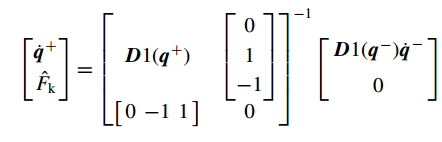
\includegraphics[width=\maxwidth{20em}]{image_0}
\end{flushleft}
\end{par}

\begin{par}
\begin{flushleft}
where D1 is 
\end{flushleft}
\end{par}

\begin{matlabcode}
disp(D1)
\end{matlabcode}
\begin{matlabsymbolicoutput}
\hskip1em $\displaystyle \begin{array}{l}
\left(\begin{array}{ccc}
I_1 +{L_1 }^2 \,m_2 +{L_1 }^2 \,m_3 +{a_1 }^2 \,m_1 +2\,m_1 \,r^2 +2\,m_2 \,r^2 +2\,m_3 \,r^2 +2\,m_1 \,r^2 \,\\
\cos \left(q_1 \right)+2\,m_2 \,r^2 \,\cos \left(q_1 \right)+2\,m_3 \,r^2 \,\\
\cos \left(q_1 \right)-2\,L_1 \,m_2 \,r-2\,L_1 \,m_3 \,r-2\,a_1 \,m_1 \,r-2\,L_1 \,m_2 \,r\,\\
\cos \left(q_1 \right)-2\,L_1 \,m_3 \,r\,\cos \left(q_1 \right)-2\,a_1 \,m_1 \,r\,\cos \left(q_1 \right) & \sigma_1  & \sigma_2 \\
\sigma_1  & m_3 \,{L_2 }^2 +m_2 \,{a_2 }^2 +I_2  & \sigma_3 \\
\sigma_2  & \sigma_3  & m_3 \,{a_3 }^2 +I_3 
\end{array}\right)\\
\mathrm{}\\
\textrm{where}\\
\mathrm{}\\
\;\;\sigma_1 =-{\left(L_2 \,m_3 +a_2 \,m_2 \right)}\,{\left(r\,\cos \left(q_2 \right)-L_1 \,\cos \left(q_1 -q_2 \right)+r\,\cos \left(q_1 -q_2 \right)\right)}\\
\mathrm{}\\
\;\;\sigma_2 =-a_3 \,m_3 \,{\left(r\,\cos \left(q_3 \right)-L_1 \,\cos \left(q_1 -q_3 \right)+r\,\cos \left(q_1 -q_3 \right)\right)}\\
\mathrm{}\\
\;\;\sigma_3 =L_2 \,a_3 \,m_3 \,\cos \left(q_2 -q_3 \right)
\end{array}$
\end{matlabsymbolicoutput}
\begin{matlabcode}

\matlabheading{Ground Collision Model}

\begin{matlabcode}
%% Ground Collision Model
syms m L I a q dq z dz [1 2]
syms r g

n = 2;
m = m.';
L = L.';
I = I.';
a = a.';
q = [q.';z.'];
dq = [dq.';dz.'];

p = cell(n,1);
p{1} = [q(3)-(a(1)-r)*sin(q(1)),q(4)-(a(1)-r)*cos(q(1))];
p{2} = [q(3)-(L(1)-r)*sin(q(1))-(L(1)-a(1))*sin(q(2)),...
        q(4)-(L(1)-r)*cos(q(1))-(L(1)-a(1))*cos(q(2))];

v = cell(n,1);
K = 0;
for i = 1:n
    v{i} = jacobian(p{i},q)*dq;
    v{i}(1) = v{i}(1)+ r*dq1;
    K = K+1/2*m(1)*v{i}.'*v{i}+1/2*dq(i).'*I(1)*dq(i);
end

Df = hessian(K,dq);
Df = simplify(expand(Df));

Ef = [q(3)-(L(1)-r)*sin(q(1))-L(1)*sin(q(2)),...
      q(4)-(L(1)-r)*cos(q(1))-L(1)*cos(q(2))];

dEf = jacobian(Ef,q);
\end{matlabcode}

\begin{par}
\begin{flushleft}
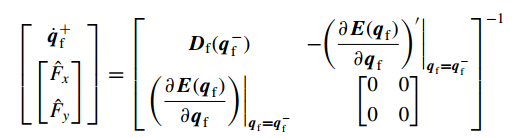
\includegraphics[width=\maxwidth{20em}]{image_1}
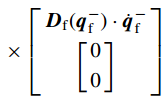
\includegraphics[width=\maxwidth{7.5em}]{image_2}
\end{flushleft}
\end{par}

\begin{par}
\begin{flushleft}
where Df and $\frac{\partial E(q_f^- )}{\partial q_f^- }$ are
\end{flushleft}
\end{par}

\begin{matlabcode}
disp(Df)
\end{matlabcode}
\begin{matlabsymbolicoutput}
\hskip1em $\displaystyle \begin{array}{l}
\left(\begin{array}{cccc}
I_1 +{L_1 }^2 \,m_1 +{a_1 }^2 \,m_1 +4\,m_1 \,r^2 +4\,m_1 \,r^2 \,\cos \left(q_1 \right)-2\,\\
L_1 \,m_1 \,r-2\,a_1 \,m_1 \,r-2\,L_1 \,m_1 \,r\,\\
\cos \left(q_1 \right)-2\,a_1 \,m_1 \,r\,\cos \left(q_1 \right) & \sigma_1  & \sigma_2  & \sigma_3 \\
\sigma_1  & m_1 \,{L_1 }^2 -2\,m_1 \,L_1 \,a_1 +m_1 \,{a_1 }^2 +I_1  & \sigma_4  & \sigma_5 \\
\sigma_2  & \sigma_4  & 2\,m_1  & 0\\
\sigma_3  & \sigma_5  & 0 & 2\,m_1 
\end{array}\right)\\
\mathrm{}\\
\textrm{where}\\
\mathrm{}\\
\;\;\sigma_1 =-m_1 \,{\left(L_1 -a_1 \right)}\,{\left(r\,\cos \left(q_2 \right)-L_1 \,\cos \left(q_1 -q_2 \right)+r\,\cos \left(q_1 -q_2 \right)\right)}\\
\mathrm{}\\
\;\;\sigma_2 =m_1 \,{\left(2\,r-L_1 \,\cos \left(q_1 \right)-a_1 \,\cos \left(q_1 \right)+2\,r\,\cos \left(q_1 \right)\right)}\\
\mathrm{}\\
\;\;\sigma_3 =m_1 \,\sin \left(q_1 \right)\,{\left(L_1 +a_1 -2\,r\right)}\\
\mathrm{}\\
\;\;\sigma_4 =-m_1 \,\cos \left(q_2 \right)\,{\left(L_1 -a_1 \right)}\\
\mathrm{}\\
\;\;\sigma_5 =m_1 \,\sin \left(q_2 \right)\,{\left(L_1 -a_1 \right)}
\end{array}$
\end{matlabsymbolicoutput}
\begin{matlabcode}
disp(dEf)
\end{matlabcode}
\begin{matlabsymbolicoutput}
\hskip1em $\displaystyle \left(\begin{array}{cccc}
-\cos \left(q_1 \right)\,{\left(L_1 -r\right)} & -L_1 \,\cos \left(q_2 \right) & 1 & 0\\
\sin \left(q_1 \right)\,{\left(L_1 -r\right)} & L_1 \,\sin \left(q_2 \right) & 0 & 1
\end{array}\right)$
\end{matlabsymbolicoutput}

\end{document}
